\documentclass[11pt,a4paper,twoside]{article}
\usepackage[margin=1in, headheight=14pt]{geometry}
\usepackage{amsfonts,amsmath,amssymb,suetterl}
\usepackage{lmodern}
\usepackage[T1]{fontenc}
\usepackage{fancyhdr}
\usepackage{float}
\usepackage[utf8]{inputenc}
\usepackage{fontawesome}
\usepackage{enumerate}
\usepackage{mathtools}
\usepackage{physics}
\usepackage{tikz}

\DeclareUnicodeCharacter{2212}{-}

\usepackage{mathrsfs}
\usepackage[nodisplayskipstretch]{setspace}

\setstretch{1.5}
\renewcommand{\footrulewidth}{0pt}

\parindent 0ex
\setlength{\parskip}{1em}

\pagestyle{fancy}
\fancyhf{}
\fancyhead[L]{\nouppercase \leftmark}
\fancyhead[R]{\thepage}

% title page
\long\def\mytitle{
	\begin{titlepage}
		\begin{center}
			\Huge Queen Mary\\
			\LARGE University of London
		\end{center}

		\vspace*{\stretch{1}}

		\begin{singlespace}
			{\centering
					{\huge\bfseries MTH5123 Differential Equations\\}
					\vspace{0.5cm}

					{\Large Lecture Notes\\}
					\vspace{0.5cm}

					{\Large Week 9}

					\vfill
					\LARGE Weini Huang
					\vspace{0.5cm}
					
					\LARGE School of Mathematical Sciences\\
					\LARGE Queen Mary University of London\\

					\vspace{0.5cm}
					\LARGE Autumn 2020\\
					}
		\end{singlespace}
	\end{titlepage}
}

\begin{document}
	\mytitle
	\section{General properties of $2 \times 2$ matrices with real entries}
	First we recall the notion of the trace and the determinant, which for $2 \times 2$ matrices are given by
	$$
	\text{Tr}A = a_{11} + a_{22}\ \text{and}\ \det A = a_{11}a_{22} − a_{12}a_{21},
	$$
	respectively. The importance of the determinant is reflected in the fact that the condition $\det A \neq 0$ ensures the possibility to find the inverse matrix $A^{-1}$,  which satisfies $A^{-1}A = AA^{-1} = I_d$. The so-called \textbf{identity matrix}
	$I_d
	=
	\begin{pmatrix}
		1 & 0\\
		0 & 1
	\end{pmatrix}
	$
	plays the same role in matrix algebra as the unity number 1 for usual numbers. Explicitly, the inverse of any $2 \times 2$ matrix with $\det A \neq 0$ is given by
	%
	\begin{equation}\label{4.7}
		A^{-1}
		= \frac{1}{\det A}
		\begin{pmatrix}
			a_{22} & -a_{12}\\
			-a_{21} & a_{11}
		\end{pmatrix}
	\end{equation}
	%
	The operation of matrix inversion is of fundamental importance, as it allows one to find the unique solution $y$ of a (non-singular) system of linear equations $A\vb{y} = \vb{b}$ as $\vb{y} = A^{-1}\vb{b}$.\\
	A vector
	$
	\vb{u}
	=
	\begin{pmatrix}
		p\\
		q
	\end{pmatrix}\neq 0
	$
	is called an eigenvector of the matrix $A$ if the equality $A\vb{u} = \lambda \vb{u}$ holds for some value of the parameter $\lambda$ known as the corresponding eigenvalue.\par
	\textbf{Theorem:}
	\begin{enumerate}
		\item There are two eigenvalues of any $2 \times 2$ matrix $A$, which are the roots of the quadratic equation
		\begin{equation}\label{4.8}
			\det (A-\lambda I_d) = \lambda^2 - \text{Tr}A\cdot \lambda + \det A = 0
		\end{equation}
		These eigenvalues are either both real or complex conjugate to each other $\bar{\lambda_1} = \lambda_2$.
		\item  If $\lambda_1 \neq \lambda_2$ then the two eigenvectors $\vb{u_1}$ and $\vb{u_2}$ are \textbf{linearly independent}\footnote{Two vectors $\vb{u_1},\ \vb{u_2}$ are linearly independent if their linear combination $c_1\vb{u_1} + c_2\vb{u_2}$ can be zero only if both $c_1$ and $c_2$ are simultaneously zero. Alternatively, two vectors are linearly dependent if there exists a constant $k \neq 0$ such that $\vb{u_2} = k\vb{u_1}$}.
		\item If $a_{12} = a_{21}$ then either $\lambda_1 = \lambda_2$ or the two eigenvectors are orthogonal, $\vb{u_1} \cdot \vb{u_2} \equiv p_1p_2 + q_1q_2 = 0$.
	\end{enumerate}
	\textbf{Proof:}\\
	\textit{This proof is not covered by the lectures and is not examinable. It is left for students who are interested to work themselves through more mathematical details.}\par
	To verify the first statement we use $\vb{u} = I_d \cdot \vb{u}\forall \vb{u}$, hence the condition of being an eigenvalue can be rewritten equivalently as
	$$
	A\vb{u} = \lambda I_d \cdot \vb{u}\quad \Leftrightarrow\quad (A − \lambda I_d) \cdot \vb{u} = 0
	$$
	for some $u \neq 0$. Now assuming $\det (A − \lambda I_d) \neq 0$ we immediately see that
	$$
	\vb{u} = (A − \lambda I_d)^{−1}\vb{0} = \vb{0},
	$$
	which is a contradiction, hence necessarily $\det (A − \lambda I_d) = 0$. Furthermore, writing
	$$
	A - \lambda I_d \equiv
	\begin{pmatrix}
		a_{11}-\lambda & a_{12}\\
		a_{21} & a_{22}-\lambda
	\end{pmatrix}
	$$
	we see that indeed
	$$
	\det (A − \lambda I_d) = (a_{11} − \lambda)(a_{22} − \lambda) − a_{12}a_{21}
	$$
	$$
	= \lambda^2 − \lambda(a_{11} + a_{22}) + (a_{11}a_{22} − a_{12}a_{21}) \equiv \lambda^2 − \text{Tr}A \cdot \lambda + \det A
	$$
	as required.\\
	To verify the second statement it is enough to demonstrate that if there exists a $k \neq 0$ such that $\vb{u_2} = k\vb{u_1}$ then necessarily $\lambda_1 = \lambda_2$. For this we consider the eigenequation $A\vb{u_1} = \lambda_1\vb{u_1}$ and multiply it with $\vb{u_2}$ from the left getting: $\vb{u_2}A\vb{u_1} = \lambda_1\vb{u_2} \cdot \vb{u_1}$. In the same way we take the second eigenequation $A\vb{u_2} = \lambda_2\vb{u_2}$ and multiply it with $\vb{u_1}$ from the left yielding $\vb{u_1}A\vb{u_2} = \lambda_2\vb{u_1} \cdot \vb{u_2}$. Subtracting both equations and using the symmetry of the scalar product $\vb{u_2} \cdot \vb{u_1} = \vb{u_1} \cdot \vb{u_2}$ yields the relation
	\begin{equation}\label{4.9}
		\vb{u_2}A\vb{u_1} - \vb{u_1}A\vb{u_2} = (\lambda_1 - \lambda_2)\vb{u_1} \cdot \vb{u_2}.
	\end{equation}
	Now, substituting here $\vb{u_2} = k\vb{u_1}$ yields on the left-hand side zero, whereas the right-hand side becomes equal to $k(\lambda_1 - \lambda_2)\vb{u_1} \cdot \vb{u_1}$. As $\vb{u_1} \neq 0$ and $k \neq 0$ we conclude that necessarily $\lambda_1 = \lambda_2$ as required. The final part of the theorem follows from the fact that for $a_{12} = a_{21}$ the left-hand side of (\ref{4.9}) is identically zero for any choice of the vectors $\vb{u_1}$ and $\vb{u_2}$ (please check!). To make the right-hand side vanishing we therefore have to require either $\lambda_1 = \lambda_2$ or $\vb{u_1} \cdot \vb{u_2} = 0$ implying the orthogonality of the eigenvectors.\par
	\textbf{Examples:}
	\begin{enumerate}[\bfseries (i)]
		\item $
		A
		=
		\begin{pmatrix}
			-4 & 6\\
			-3 & 5
		\end{pmatrix}
		$
		with $\lambda_1 = 2$, $\vb{u_1} = \begin{pmatrix} 1 \\ 1\end{pmatrix}$ and $\lambda_2 = -1$,
		$
		\vb{u_2}
		=
		\begin{pmatrix}
			2\\
			1
		\end{pmatrix}
		$.
		\item $
		A
		=
		\begin{pmatrix}
			0 & 1\\
			-2 & 2
		\end{pmatrix}
		$
		with $\lambda_1 = 1 + i$,
		$
		\vb{u_1} = 
		\begin{pmatrix}
			1\\
			1+i
		\end{pmatrix}
		$
		and $\lambda_2 = 1-i$,
		$
		\vb{u_2}
		=
		\begin{pmatrix}
			1\\
			1-i
		\end{pmatrix}
		$.
	\end{enumerate}
	\textbf{Note:} Eigenvectors are determined up to a nonzero factor.
	The last useful property needed to be mentioned is as follows: Suppose a matrix $A$ has two distinct eigenvalues $\lambda_1 \neq \lambda_2$ and an associated pair of two linearly independent eigenvectors
	$
	\vb{u_1} = 
	\begin{pmatrix}
		p_1\\
		q_1
	\end{pmatrix} \neq 0
	$
	and
	$
	\vb{u_2} = 
	\begin{pmatrix}
		p_2\\
		q_2
	\end{pmatrix} \neq 0
	$.
	Then the matrix
	$
	U =
	\begin{pmatrix}
		p_1 & p_2\\
		q_1 & q_2
	\end{pmatrix}
	$
is nonsingular, that is $\det U \neq 0$, and therefore can be inverted giving $U^{-1}$. Moreover, the matrix $U^{-1}AU$ turns out to be always diagonal and equal to
$
\begin{pmatrix}
	\lambda_1 & 0\\
	0 & \lambda_2
\end{pmatrix}
$.
The last fact follows from
$$
AU=
\begin{pmatrix}
	a_{11} & a_{12}\\
	a_{21} & a_{22}
\end{pmatrix}
\begin{pmatrix}
	p_1 & p_2\\
	q_1 & q_2
\end{pmatrix}
=
\begin{pmatrix}
	\lambda_1p_1 & \lambda_2p_2\\
	\lambda_1q_1 & \lambda_2q_2
\end{pmatrix}
=
U\begin{pmatrix}
	\lambda_1 & 0\\
	 & \lambda_2
\end{pmatrix}
$$
where we have used that the condition $A\vb{u} = \lambda \vb{u}$ for
$
\vb{u} =
\begin{pmatrix}
	p\\
	q
\end{pmatrix}
$
is equivalent to $a_{11}p_i + a_{12}q_i = \lambda p_i$ and $a_{21}p_i + a_{22}q_i = \lambda q_i$, $i = 1,\ 2$. Now we will use these properties for solving the system of linear ODE’s.
%
\section{General analysis of the linearised ODE system for}
$$D = (\textbf{Tr}A)^2 - 4\det A \neq 0$$
Solving the characteristic equation $\det (A − \lambda I_d) = \lambda^2 − \text{Tr}A \cdot \lambda + \det A = 0$. for $\lambda$ yields $\lambda = \frac{\text{Tr}A}{2}\pm \frac{1}{2}\sqrt{(\text{Tr}A)^2 - 4\det A}$. This shows that in this case we must have two distinct roots. In the case $D = (\text{Tr}A)^2 − 4 \det A > 0$ these roots are real,
$$
\lambda_1 = \frac{1}{2}(\text{Tr}A + \sqrt{D}) > \lambda_2 \frac{1}{2}(\text{Tr}A - \sqrt{D}),
$$
hence the corresponding eigenvectors $\vb{u_1}$ and $\vb{u_2}$ must also be real and linearly independent. In the opposite case $D = (\text{Tr}A)^2 − 4 \det A < 0$ the two roots are complex conjugate,
$$
\lambda_1 = \frac{1}{2}(\text{Tr}A + i\sqrt{|D|}),\ \lambda_2 = \frac{1}{2}(\text{Tr}A - i\sqrt{|D|}),
$$
and the eigenvectors may be complex but are still linearly independent, as $\lambda_1 \neq \lambda_2$. Given a pair of linearly independent vectors we know that we can write an arbitrary vector of the same dimension as a linear combination of these two vectors.\\
We can thus look for a solution
$
\vb{y} \equiv
\begin{pmatrix}
	y_1\\
	y_2
\end{pmatrix}
$
of the ODE system
$
\begin{pmatrix}
	\dot{y_1}\\
	\dot{y}
\end{pmatrix}
= A
\begin{pmatrix}
	y_1\\
	y_2
\end{pmatrix},\quad
A =
\begin{pmatrix}
	a_{11} & a_{12}\\
	a_{21} & a_{22}
\end{pmatrix}
$
in the form of $y = c_1\vb{u_1} + c_2\vb{u_2}$, where the coefficients $c_1$ and $c_2$ are assumed to depend on $t$. We then have $\dot{\vb{y}} = \dot{c_1}\vb{u_1} + \dot{c_2}\vb{u_2}$, which by substituting into the above ODE system gives the chain of identities
\begin{equation}\label{4.10}
	\dot{c_1}\vb{u_1} + \dot{c_2}\vb{u_2} = A(c_1\vb{u_1} + c_2\vb{u_2}) = c_1\lambda_1\vb{u_1} + c_2\lambda_2\vb{u_2}
\end{equation}
or, rearranging,
\begin{equation}\label{4.11}
	(\dot{c_1} - \lambda_1c_1)\vb{u_1} = -(\dot{c_2} - c_2\lambda_2)\vb{u_2} , 
\end{equation}
which must hold at any moment of time $t$. Using linear independence of the two eigenvectors we conclude that simultaneously we must have
$$
\dot{c_1} = \lambda_1c_1\ \text{and}\ \dot{c_2} = \lambda_2c_2.
$$
These separable equations are immediately solved to produce
\begin{equation}\label{4.12}
	c_1(t) = c_1e^{\lambda_1t}\ c_2(t) = c_2e^{\lambda_2t},
\end{equation}
where $c_{1,2}$ are constants. We conclude that the general solution to this ODE system in such a case is given by
\begin{equation}\label{4.13}
	\vb{y}(t) = c_1e^{\lambda_1t}\vb{u_1} + c_2e^{\lambda_2t}\vb{u_2}.
\end{equation}
For any initial value problem with the ODE system,
$
\begin{pmatrix}
	\dot{y_1}\\
	\dot{y}
\end{pmatrix}
= A
\begin{pmatrix}
	y_1\\
	y_2
\end{pmatrix},\quad
A =
\begin{pmatrix}
	a_{11} & a_{12}\\
	a_{21} & a_{2}
\end{pmatrix},
$
the values of $c_1$ and $c_2$ will be determined by the initial conditions $y_1(0) = a$ and $y_2(0) = b$ and the eigenvectors
$
\vb{u_1} = 
\begin{pmatrix}
	p_1\\
	q_1
\end{pmatrix}
$
and
$
\vb{u_2}=
\begin{pmatrix}
	p_2\\
	q_2
\end{pmatrix}
$
as, according to (\ref{4.13}), $a = c_1p_1 + c_2p_2,\ b = c_1q_1 + c_2q_2$.\par
\textbf{Example:}\\
Consider the ODE system,
$
\begin{pmatrix}
	\dot{y_1}\\
	\dot{y}
\end{pmatrix}
= A
\begin{pmatrix}
	y_1\\
	y_2
\end{pmatrix},\quad
A =
\begin{pmatrix}
	a_{11} & a_{12}\\
	a_{21} & a_{22}
\end{pmatrix}
$
with the particular choice of $A$
\begin{equation}\label{4.14}
	\begin{pmatrix}
		\dot{y_1}\\
		\dot{y}
	\end{pmatrix}
	= A
	\begin{pmatrix}
		y_1\\
		y_2
	\end{pmatrix},\ 
	A =
	\begin{pmatrix}
		-4 & 6\\
		-3 & 5
	\end{pmatrix}.
\end{equation}
In exercise (i) on p.5 we have found that $\lambda_1 = 2,\
\vb{u_1} = 
\begin{pmatrix}
	1\\
	1
\end{pmatrix}
$
and
$
\lambda_2,\ 
\vb{u_2} = 
\begin{pmatrix}
	2\\
	1
\end{pmatrix}
$.
According to (\ref{4.13}), the solution is given by
$$
\begin{pmatrix}
	y_1\\
	y_2
\end{pmatrix}
= c_1e^{2t}
\begin{pmatrix}
	1\\
	1
\end{pmatrix}
+ c_2e^{-t}
\begin{pmatrix}
	2\\
	1
\end{pmatrix}.
$$
The initial conditions $x(0) = a,\ y(0) = b$ can now be written as
$$
a = c_1 + 2c_2,\ b = c_1 + c_2 .
$$
Solving these equations we get $c_2 = a - b,\ c_1 = 2b - a$ so that the explicit expressions for the time dependence of the coordinates in the $(y_1, y_2)$ plane are given by
$$
y_1 = (2b-a)e^{2t} + 2(a-b)e^{-t},\ y_2 = (2b-a)e^{2t} + (a-b)e^{-t}.
$$
\section{Phase portraits for linearised systems}
The eigenvalues of the linearised system are $lambda = \frac{\text{Tr}A}{2}\pm \frac{1}{2}\sqrt{D}$, where $D = (\text{Tr}A)^2 - 4 \det A$. We can classify the phase portraits of our linear systems based the different situations of the eigenvalues.
\subsection{Transformation of phase portraits between coordinates through invariant manifolds}
In our example in last section, we have two distinct real eigenvalues, where $\lambda_1 = 2$ and $\lambda_2 = −1$. How do the trajectories look like for different initial conditions, which means when $a, b$ have different values?\\
Consider when $b = a/2$, which implies $y_1 = ae^{-t},\ y_2=\frac{a}{2}e^{-t}$. We conclude that $y_2 = y_1/2\ \forall t$, i.e., this trajectory corresponds to motion along a straight line with slope $1/2$ towards the origin (since both $y_1$ and $y_2$ tend to zero for $t \to \infty$). Similarly, for $b = a$ we have $y_2 = y_1 = ae^{2t}\ \forall t$, which describes motion along a straight line away from the origin. These two special straight lines are known as invariant manifolds, which correspond to the two lines on top of the two eigenvectors. They intersect at the origin and partition the phase space, which is $(y1, y2)$ plane, into four sectors, see Fig.\ref{f:4.1} (left). Asymptotically the trajectories which start from initial conditions such that $b > a/2$ tend to approach to the line $y_2 = y_1 \to +\infty$ for $t \to \infty$, whereas the trajectories with initial conditions such that $b < a/2$ tend to approach to the line $y_2 = y_1 \to -\infty$ for $t \to \infty$.\\
In the above example we have fully understood the structure of the trajectories in the $(y_1, y_2)$ phase space, which is called a phase portrait. This picture is looking rather complicated, but it simplifies if we transform into specific coordinates. For this purpose we introduce the vector
$
\vb{\tilde{y}}\equiv
\begin{pmatrix}
	\tilde{y_1}\\
	\tilde{y_2}
\end{pmatrix}
$
of new coordinates $\tilde{y_1}, \tilde{y_2}$ related to the vector of old coordinates
$
\vb{y} =
\begin{pmatrix}
	x\\
	y
\end{pmatrix}
$
via 
$
\vb{\tilde{y}} = U^{-1}\vb{y}
$
or equivalently $\vb{y} = U\tilde{y}$. The columns of the $2 \times 2$ matrix $U$ are chosen to be the eigenvectors
$
\vb{u_1} = 
\begin{pmatrix}
	1\\
	1
\end{pmatrix}
$
and
$
\vb{u_2} = 
\begin{pmatrix}
	2\\
	1
\end{pmatrix}
$,
which implies
\begin{figure}[!h]
	\centering
		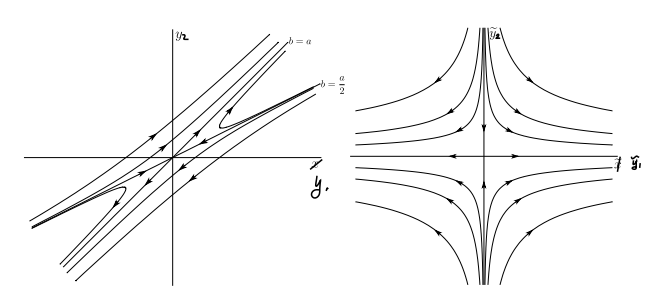
\includegraphics[width=0.75\textwidth]{figure/fig21_4_1.PNG}
		\caption{Phase portraits of the ODE (\ref{4.14}) in old (left) and in new (right) coordinates.}\label{f:4.1}
\end{figure}
$
U^{-1} = 
\begin{pmatrix}
	1 & -2\\
	-1 & 1
\end{pmatrix}
$.
This yields the chain of identities
\begin{equation}\label{4.15}
	\frac{d}{dt}\vb{\tilde{y}} = U^{-1}\frac{d}{dt}\vb{y} = U^{-1}A\vb{y} = U^{-1}AU\vb{\tilde{y}}
\end{equation}
and accordingly the system of ODEs in new coordinates
\begin{equation}\label{4.16}
	\frac{d}{dt}\vb{\tilde{y}}, = \tilde{A}\vb{\tilde{y}},\ \tilde{A} = U_{-1}AU =
	\begin{pmatrix}
		2 & 0\\
		0 & -1
	\end{pmatrix}.
\end{equation}
%
Hence, this system is equivalent to $\dot{\tilde{y_1}} = 2 \tilde{y_1},\ \dot{\tilde{y_2}} = -\tilde{y_2}$. Specifying initial conditions in new coordinates as $\tilde{y_1}(0) = \tilde{a}, \tilde{y_2}(0) = \tilde{b}$ we solve these equations to $\tilde{y_1}(t) = \tilde{a}e^{2t},\ \tilde{y_2}(t) = \tilde{b}e^{-t}$. Eliminating the time variable $t$ we find the trajectories to be given by $\tilde{y_2} = \tilde{b}(\frac{\tilde{y_1}}{a})^{-1/2}$ if $\tilde{a} \neq 0$ and $\tilde{y_1} = 0$ if $\tilde{a} = 0$. Moreover, for $t \to \infty$ we have $\tilde{y_2} \to 0$ whereas $\tilde{y_1} \to \infty$ for $\tilde{a} > 0$ and $\tilde{y_1} \to -\infty$ for $\tilde{a} < 0$. This allows us to sketch the phase portrait given in Fig. \ref{f:4.1} (right).\\
Comparing these two phase portraits in old and new coordinates we see that qualitatively they look similar. However, the one in old coordinates $(y_1, y_2)$ is a kind of rotated, twisted and stretched version of the one in new coordinates $\tilde{y_1}, \tilde{y_2}$. In particular, in new coordinates the important straight lines which partition the plane into four sectors coincide with the two coordinate axes simplifying the picture. These two pictures are called topologically equivalent meaning that one can be transformed into the other by a continuous set of transformations without the need to cut or tear the plane apart (imagine the plane to be made of plasticine, which can be easily distorted). Phase portraits for other types of systems may not be deformed that way and are then of a different topological type, as we shall see in the next example.
\end{document}